 \documentclass{article}
\usepackage[utf8]{inputenc}
\usepackage[top=3cm, bottom=3cm, left=3cm,right=3cm]{geometry}
%\usepackage[numbers,round]{natbib}
\usepackage{natbib}
\setcitestyle{aysep={}} 
\usepackage{graphicx}
\usepackage{color}
\usepackage{amsmath}
\usepackage{setspace}
\usepackage{amsmath}
\usepackage{mathtools}
\usepackage{bbm}
\usepackage{float}
\usepackage{hyperref}
\usepackage[super]{nth}

\parindent0cm
\parskip0.5cm
\hyphenpenalty=10000
\pretolerance=10000
\usepackage{lineno}
\linenumbers

\def\packagename{ValidateDating}
\def\packageurl{\texttt{https://github.com/xavierdidelot/ValidateDating}}

\makeatletter
\newcommand{\customlabel}[2]{
\protected@write \@auxout {}{\string \newlabel {#1}{{#2}{}}}}
\makeatother

\renewcommand\footnote[2][]{\relax}

\begin{document}
{\Large Validation of dated phylogenies in microbial population genetics}


\vspace*{2cm}
Xavier Didelot$^{1,*}$, Paolo Ribeca$^{2,3}$, ...

\vspace*{2cm}
$^1$ School of Life Sciences and Department of Statistics, University of Warwick, United Kingdom\\\\
$^2$ UK Health Security Agency, London, United Kingdom\\\\
$^3$ Biomathematics and Statistics Scotland, The James Hutton Institute, Edinburgh, United Kingdom\\\\
$^*$ Corresponding author. Tel: 0044 (0)2476 572827. Email: \verb+xavier.didelot@gmail.com+

%\newpage
%\section*{ABSTRACT}
%TODO

\newpage
\section*{INTRODUCTION}

Dated phylogenies, also known as tip-calibrated, time-stamped or time-calibrated phylogenies, have become a ubiquitous tool in the study of microbial population genetics 
\citep{Drummond2003,Biek2015,rieuxInferencesTipcalibratedPhylogenies2016}. In a dated phylogeny, the branch lengths are measured in a unit of time, for example years or days,
rather than a unit of evolution as in a standard phylogeny. Consequently, the tips of a dated phylogeny are aligned with the (typically known) dates of sampled genomes and
the internal nodes are aligned with the (typically inferred) dates of common ancestors between the genomes.
Many tools exist to build dated phylogenies, either from a sequence alignment using for example BEAST \citep{Suchard2018} or BEAST2 \citep{Bouckaert2019}, or by
dating the nodes of a standard phylogeny, using for example 
LSD \citep{To2016}, node.dating \citep{Jones2017}, treedater \citep{Volz2017}, BactDating \citep{Didelot2018} and TreeTime \citep{Sagulenko2018}.

There are several factors that can invalidate the results. 
See \citep{tongComparisonMethodsEstimating2018} for a list.
This includes the confounding effect that population structure can have on dating \citep{Murray2016}.
It also includes any incorrect assumptions made when running a dating analysis, for example using an inappropriate clock model. 

Validation is not the same as model comparison \citep{Baele2012,Li2012,bouckaertBModelTestBayesianPhylogenetic2017}. 
Also validation is not the same as testing significance of temporal signal \citep{Duchene2015a,Duchene2020}.

\section*{MATERIALS AND METHODS}

\subsection*{General approach}

\begin{figure}[t!]
\begin{center}
A\hspace*{6cm}B\hspace*{6cm}~\\
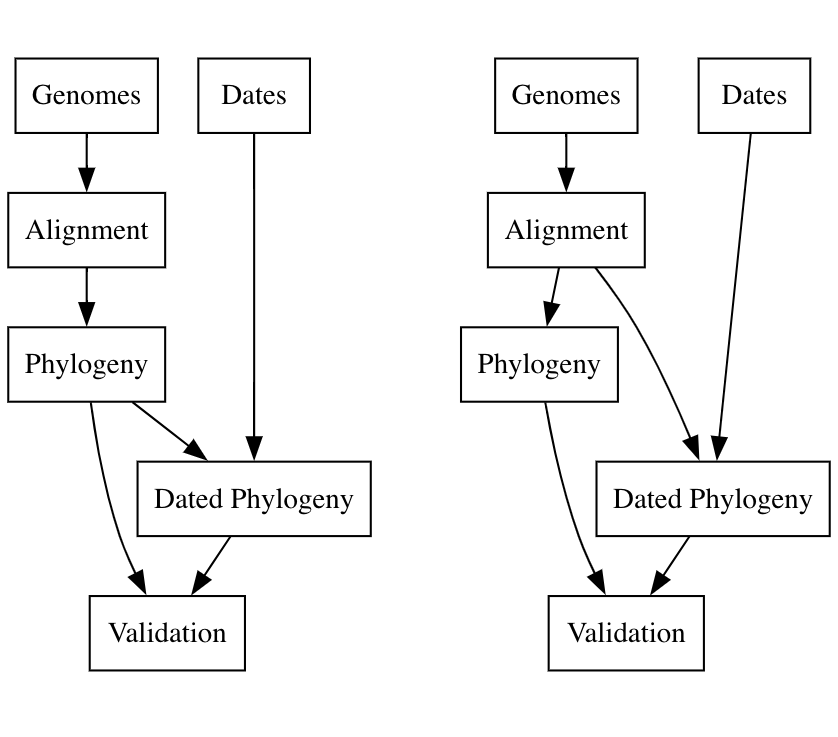
\includegraphics[width=10cm]{fig1.png}
\end{center}
\caption{(A) General approach for validation of a dated phylogeny built by dating the nodes of a standard phylogeny. (B) General approach for validation of a dated phylogeny built directly from a sequence alignment.
\label{fig:approach}}
\end{figure}

Comparison of dated phylogeny $\mathcal{D}$ with undated phylogeny $\mathcal{L}$. Especially makes sense when dated phylogeny is built from the undated phylogeny (Figure \ref{fig:approach}A) and so we focus on this here. But can also be used for methods that build a dated phylogeny directly from the alignment (Figure \ref{fig:approach}B).

Let $d_i$ be the duration of a given branch in $\mathcal{D}$ and $l_i$ be the number of substitutions on the corresponding branch of $\mathcal{L}$, that is the branch that separates the leaves in the same way. There is a unique corresponding branch in $\mathcal{L}$ for all branches in $\mathcal{D}$ except for the two branches $a$ and $b$ connected to the root of $\mathcal{D}$ for which there is only a single corresponding branch $x$. We therefore split the substitutions on $x$ proportionally between the two branches $a$ and $b$ by defining:

\begin{equation}
l_a = \frac{l_x d_a}{d_a+d_b}\mathrm{~and~}l_b = \frac{l_x d_b}{d_a+d_b}
\end{equation}

The distribution of $l_i$ given $d_i$ is given by the molecular clock model. For example, if we consider a discrete strict clock model \citep{Zuckerkandl1962} with rate $\mu$ then we have that 
substitutions occur on the branch as a Poisson process with rate $\mu$ and therefore:

\begin{equation}
l_i \sim \mathrm{Poisson}(d_i \mu)
\label{eq:strict}
\end{equation}

In this case the distribution of $l_i$ is discrete, but let us for know consider that the distribution
is continuous and we will return later to the discrete case. 
Several examples of continuous clock models have been previously described \citep{Didelot2021},
but here we consider the general case where
$F_i(l_i)$ is the cumulative distribution function of $l_i$ given $d_i$.
Let $u_i$ denote the uniform residual for the observation $l_i$, defined as:

\begin{equation}
u_i=F_i(l_i)=p(L_i\leq l_i|d_i)
\label{eq:unif-resid}
\end{equation}

If the model is valid, then the uniform residual $u_i$ 
should be distributed as Unif(0,1), because for any random variable $X$ with cumulative distribution function $F$ we have that $U=F(X)$ is Unif(0,1). 
We can also define normal residuals $n_i$, analogous to the residuals commonly used in 
regression models, by transforming with the inverse of the cumulative distribution function $\Phi$ 
of a Normal(0,1) random variable:

\begin{equation}
n_i=\Phi^{-1}(u_i)
\label{eq:norm-resid}
\end{equation}

If the model is valid, then the normal residual $n_i$ should be distribution
as Norm(0,1). 

TODO DISCRETE CASE

\section*{RESULTS}

TODO

\section*{DISCUSSION}

TODO

\section*{ACKNOWLEDGEMENTS}

We acknowledge funding from the National Institute for Health Research (NIHR) Health Protection Research Unit in Genomics and Enabling Data.

\newpage
\bibliographystyle{mbe}
\bibliography{/Users/u1775021/all.bib}
%\bibliography{biblio}

\pagenumbering{gobble}
\newpage
%Supplementary Material
\setcounter{figure}{0}
\setcounter{table}{0}
\makeatletter 
\renewcommand{\thefigure}{S\@arabic\c@figure} 
\renewcommand{\thetable}{S\@arabic\c@table} 
\makeatother

\end{document}

%# Done so far
%
%- Dating via node.dating, BactDating, treedater, TreeTime and LSD2
%- Reproduce confounding effect described by Murray2016 on similar coalescent simulation, cf `confounding.Rmd`
%- Ruled out possible problem in phylogenetics since working directly with trees, not genetic data
%- Ruled out possible problem with root identification (ie consider root known)
%- Ruled out possible problem with multifurcation at the root (relaxed this in simulation)
%- More general version in `confounding-simstructure.Rmd` in which sampling dates do not have to be identical, and population sizes do not have to be constant. Simulation code is in `simStructure.R`, uses some of mlesky code for simulation of non-homogeneous Poisson coalescent process.
%- Difficult to get confusion using DetectImports simulations, cf `confounding-detectimports.Rmd`. May be because confusion only happens when sampling dates are biased, whereas DetectImports assumes sampling according to relative prevalence of populations
%- A Mendel test has been proposed to detect when confounding might happen, but this will flag an issue even if there is no structure and no problem with dating, cf `struture-test.Rmd`
%- When there is no confounding issue but the temporal signal is weak, eg because all sampling dates are the same or very similar, see `run-nosignal.Rmd`. Estimate incorrectly high clock rate. But the permutation test shows this is not to be trusted.
%

%Urgent TODO list
%Function for making a resDating object from a dated tree and a standard phylogeny which could be unrooted
%Use this eg in perfect residuals vignette and also the runDating subfunctions
%Also use in readme?
%Allow root inference
%Clock relaxation only works in BactDating currently
%Investigate false positives

%# Old to do
%
%- Propose new test to detect when the confounding problem happens
%- Implemented first naive idea of doing a Krukal-Wallis test comparing the dates on the left and right for each node, cf testConfounding.R. Get false positive in structure-test.Rmd. Need better test, accounting for branch lengths. Maybe idea of using pseudo-residuals.
%- Propose a solution to when the confounding problem happens, maybe via removal of some leaves until test satisfied
%- Is permutation test useful?
%- Is clustered permutation test useful?
%- Comparison with run in which all leaves have same date. Attractive as only need to run once. Use DIC or something else?
%- Use better Bayesian model comparison methods?
%- Use Bayesian model criticism approach? Maybe using posterior predictive p-values?
%- Effect of relaxed clock models, especially ARC.
%- Effect of priors, especially on tree (constant effective population size as in Murray2016) but also others.
%- Apply to real data. May be able to reuse data from Holden2013, cf Fig S4 in Murray2016.
%
%# Some ideas
%
%- Fit with all dates equal using modified BactDating. Need to add move to scale up tree and down rate simultaneously, and vice versa. Consider prior effect. Given this fit, do posterior predictive test to see if there is a temporal signal. 
%- Joint model with and without temporal signal, to estimate Bayes Factor directly with rjMCMC. Current moves on sampling times could be starting point. 
%- Show confounding only happens when we have structure plus uneven sampling between structure component. Develop test for this based on undated phylgeny plus sampling dates. Bit like treeBreaker with continuous phenotype representing sampling dates.
%- Can a relaxed clock with high relaxation parameter equate a lack of temporal signal? What happens in ARC if omega is very high?
%- Alternate method to simulate confounding tree: generate very large phylogeny and subsample from large clusters within in
%- Shiny app

